% !TEX encoding = IsoLatin2  % notwendige Zeile f"ur Mac-Benutzer (muss als Kommentar stehen); Windows-Benutzer k"onnen die Zeile l"oschen.

% LaTeX-Vorlage Version 3.1,  Juli 2011
% erstellt von Dr. Andreas Drauschke (andreas.drauschke@technikum-wien.at) und Dr. Susanne Teschl (susanne.teschl@technikum-wien.at)
% geringf"ugig adaptiert von Harald Stockinger (harald.stockinger@technikum-wien.at)


\documentclass[a4paper,bibtotoc,oneside]{scrbook}
% F"ur kurze Arbeiten w"are auch die Dokumentklasse "scrartcl" ausreichend. In diesem Fall ist "section" die h"ochste Ebene ("chapter" gibt es dann nicht).
% \documentclass[a4paper,bibtotoc,oneside]{scrartcl}


% verlinkte Querverweise im pdf
\usepackage{hyperref}
\usepackage[utf8x]{inputenc}
% deutsche Anpassungen
% \usepackage[ansinew]{inputenc}
\usepackage[T1]{fontenc}
\usepackage[ngerman]{babel}
% mathematische Symbole
\usepackage{amsmath,amssymb,amsfonts,amstext}

\usepackage{caption}
%tabellen

% Kopfzeilen frei gestaltbar
\usepackage{fancyhdr}
\lfoot[\fancyplain{asdf}{}]{\fancyplain{}{}}
\rfoot[\fancyplain{}{}]{\fancyplain{}{}}
\cfoot[\fancyplain{}{\footnotesize\thepage}]{\fancyplain{}{\footnotesize\thepage}}
\lhead[\fancyplain{}{\footnotesize\nouppercase\leftmark}]{\fancyplain{}{}}
\chead{}
\rhead[\fancyplain{}{}]{\fancyplain{}{\footnotesize\nouppercase\sc\leftmark}}

% Farben im Dokument m"oglich
\usepackage{color}

% Schriftart Helvetica
\usepackage{helvet}
\renewcommand{\familydefault}{cmss}

% Graphiken einbinden: hier f"ur pdflatex
\usepackage[pdftex]{graphicx}

\usepackage{array}

% H"ohe und Breite des Textk"orpers etwas gr"osser definieren
\setlength{\textheight}{225mm}
\setlength{\textwidth}{1.05\textwidth}

% weniger Warnungen wegen "uberf"ullter Boxen
\tolerance = 9999
\sloppy

% Anpassung einiger "Uberschriften
\renewcommand\figurename{Abbildung}
\renewcommand\tablename{Tabelle}

% %footers and headers
% % \usepackage{fancyhdr}
% % \pagestyle{fancy}
% \lhead{\studiumshort}
% \chead{}
% \rhead{\fachnameshort}
% \lfoot{\teilnehmeronenachname, \teilnehmertwonachname}
% % \cfoot{erstellt am: \today}
% \rfoot{\thepage}
% \renewcommand{\headrulewidth}{0.5pt}
% \renewcommand{\footrulewidth}{0.5pt}

\begin{document}

% Kopf- und Fusszeilen initiieren
\pagestyle{fancy}

% Deckblatt:
\thispagestyle{empty}
\begin{picture}(0,0)
\color{white}\sffamily
\put(-101,-412){
\includegraphics[width=1.002\paperwidth]{./picture/LPS_2011.pdf}}
\put(220,-670){
\includegraphics[width=0.5\textwidth]{./picture/FHTW_Logo_4c.pdf}}
\put(-30, -20){\bfseries\huge SEMINARARBEIT}
% Titel des Studienganges einf"ugen:
\put(-30,-50){\Large im Studiengang BEL3}
% Titel der Lehrveranstaltung einf"ugen:
\put(-30,-70){\Large Lehrveranstaltung Audiotechnik}
\color{black}
% Titel der Arbeit einf"ugen:
% Die Minipage wird gesetzt, damit auch mehrzeilige Titel m"oglich werden.
\put(-32,-350){
\begin{minipage}{13cm}
\bfseries\huge D-Verstärker
\end{minipage}
}
% Name der Autorin/des Autors eingeben:
% Personenkennzeichen der Autorin/des Autors eingeben:
\put(-30,-450){\large Ausgeführt von:\ Christian Schwarzgruber}
\put(+54,-470){\large \ Alexander Rössler}
\put(-30,-490){\large Matrikelnummer: 1110254027}
\put(+63,-510){\large 1110254020}
% Name der Begutachterin/des Begutachters eingeben:
\put(-30,-550){\large Begutachter: Michael Windisch}
\put(-30,-590){\large Wien, \today} % das Datum des letzten Kompilierens wird automatisch eingesetzt
\end{picture}

\newpage



% \section*{Kurzfassung}\thispagestyle{empty}
% Text Text Text Text Text Text Text Text Text Text Text Text Text Text Text Text Text Text Text Text Text Text Text Text
% Text Text Text Text Text Text Text Text Text Text Text Text Text Text Text Text Text Text Text Text Text Text Text Text
% Text Text Text Text Text Text Text Text Text Text Text Text Text Text Text Text Text Text Text Text Text Text Text Text
% Text Text Text Text Text Text Text Text Text Text Text Text Text Text Text Text Text Text Text Text Text Text Text Text
% Text Text Text Text Text Text Text Text Text Text Text Text Text Text Text Text Text Text Text Text Text Text Text Text ...
% \\[3\baselineskip] % Abstand zum Abstract (evtl. "andern)
% \section*{Abstract}
% Text Text Text Text Text Text Text Text Text Text Text Text Text Text Text Text Text Text Text Text Text Text Text Text
% Text Text Text Text Text Text Text Text Text Text Text Text Text Text Text Text Text Text Text Text Text Text Text Text
% Text Text Text Text Text Text Text Text Text Text Text Text Text Text Text Text Text Text Text Text Text Text Text Text
% Text Text Text Text Text Text Text Text Text Text Text Text Text Text Text Text Text Text Text Text Text Text Text Text
% Text Text Text Text Text Text Text Text Text Text Text Text Text Text Text Text Text Text Text Text Text Text Text Text ...
% \newpage


\tableofcontents\thispagestyle{empty}
\newpage

\setcounter{page}{1}

% Falls die Kapitel"uberschriften zu lang f"ur die Kopfzeile oder das Inhaltsverzeichnis sind, so erzielt man
% dort Kurzformen der Kapitelbezeichnungen mittels:
% \chapter[Kurzform]{Lange "Uberschrift}
\chapter[Recherche über Klasse D-Verstärker]{D-Verstärker}
Es gibt eine große Vielzahl von verschiedenst Implementierten D-Verstärker, doch besitzen sie allesamt die selben
Grundbauelement, diese sind...fortsetzung folgt :-)
\section[Erster Abschnitt]{"Uberschrift des ersten Abschnitts}

Text Text Text Text Text Text Text Text Text Text Text Text Text Text Text Text Text Text Text Text Text Text Text Text ...

\subsection[Erster Unterabschnitt]{"Uberschrift des ersten Unterabschnitts}

Text Text Text Text Text Text Text Text Text Text Text Text Text Text Text Text Text Text Text Text Text Text Text Text ...

\subsubsection[Erster Unter-Unterabschnitt]{Und noch eine Ebene tiefer}

Im Folgenden werden einige Beispiele f"ur h"aufig gebrauchte Anweisungen gegeben. Sie dienen als Einstiegshilfe in
\LaTeX\ und
nicht als starre Formatvorgaben.
\\[2\baselineskip]
Hier wird auf Abbildung~\ref{Abb1} verwiesen.
\begin{figure}[htbp]
\centering
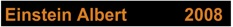
\includegraphics[width=75mm]{./picture/Buchruecken}
\caption[Beschriftung eines Buchr"uckens.]{Beispiel f"ur die Beschriftung eines Buchr"uckens.}\label{Abb1}
\end{figure}
Tabelle~\ref{Tab1} ist ein Beispiel daf"ur, wie eine Tabelle aussehen k"onnte.
\begin{table}[htbp]
\centering
\begin{tabular}{ | c | c | c | }\hline
{\bf Datum} & {\bf Thema} & {\bf Raum}\\ \hline
\hline
20. 08. 2008 & Graphentheorie & HS 3.13\\ \hline
01. 10. 2008 & Biomathematik & HS 1.05\\ \hline
\end{tabular}
\caption[Semesterplan "`Angewandte Mathematik"'.]{Beispiel f"ur einen Semesterplan "`Angewandte Mathematik"'.}\label{Tab1}
\end{table}
\chapter{Seminarbuch}
\begin{table}[htbp]
  \centering
  \captionsetup{margin=1pt,font=small,labelfont=bf}
  \caption{Arbeitsaufwand}
    \begin{tabular}{| c | c| c | c |}\hline
    {\bf Arbeitstag} &{\bf Tätigkeit} &{\bf Arbeitszeit(h)} &{\bf Dokumentation(h)} \\\hline
    \hline
    1. Tag   & Recherche im Internet über D-Verstärker   & 1   & 1 \\
    2. Tag   & Durchführung Übung 2 Transistoren Messung  & 4   & 4 \\
    3. Tag   & Durchführung Übung 3 Signalkennwerte Messung   & 4   & 7 \\
    \hline
    \textbf{Gesamt}   & \textbf{}    & \textbf{12}   & \textbf{14} \\
    \hline
    \end{tabular}%
  \label{tab:addlabel}%
\end{table}%
\noindent
Nun ein Beispiel f"ur eine abgesetzte Formel:
\begin{equation}
x =  - \frac{p}{2} \pm \sqrt{\left(\frac{p}{2}\right)^2 - q}.
\end{equation}
Und eine mehrzeilige Formel:
\begin{eqnarray}
f(t)&=& t^2 \label{For1},\\
g(t) &=& t-1.
\end{eqnarray}
Hier wird auf die Formel (\ref{For1}) verwiesen. \\

\noindent
So kann zum Beispiel ein \glqq Source-Code\grqq\  angegeben werden:
\begin{verbatim}
for (i=1; i < 10; i++) {...}
\end{verbatim}

\noindent
Hier ist ein Hyperlink auf die  \href{http://www.technikum-wien.at}{Homepage} der FH Technikum Wien. Email-Adressen k"onnen so verlinkt werden: \href{mailto:homer.simpson@springfield.com}{\texttt{homer.simpson@springfield.com}}\\

\noindent
In der Bibliothek der Fachhochschule Technikum Wien gibt es verschiedene einf"uhrende B"ucher zum Thema \glqq \LaTeX \grqq, zum Beispiel \cite{kop05}, \cite{wil06} oder \cite{mgb+05d} (deutsche Version) bzw. \cite{mgb+04e} (englische Version). Empfehlenswerte Skripten f"ur \LaTeX-Einsteiger sind z.B. \cite{mj00} und \cite{mj95}. Sie sind frei im Internet verf"ugbar.


% Literaturverzeichnis
% Das Literaturverzeichnis kann auch nach einem allf"alligen Anhang positiioniert werden (siehe "`Leitfaden f"ur Bachelor- und Diplomarbeiten"', Version 2.0, Abschnitt 2.9).

% M"oglichkeit 1: Erzeugung des Literaturverzeichnisses mit BibTeX:
% Die Quellen sind in der Datei *.bib (hier Literatur.bib) einzugeben. Danach muss diese Vorlage einmal geTeXt werden,
dann BibTeX angewendet werden und
% anschliessend nochmals zweimal geTeXt werden.
% Im Text erfolgt die Zitierung mit dem Anker-Schl"usselwort, z.B. \cite{kop05}.
\bibliographystyle{IEEEtran}
\bibliography{Literatur}

% M"oglichkeit 2: Erzeugung eines Literaturverzeichnisses ohne BibTeX:
%\begin{thebibliography}{99}
%\bibitem[kop05]{kop05}
%H.~Kopka, {\em LaTeX, Band 1: Einf"uhrung}, Pearson Studium, M"unchen, 3.~Auflage, 2005.
%\bibitem[knu98]{knu98}
%F.~Mittelbach, M.~Goossens, J.~Braams, D.~Carlisle, and Ch. Rowley, {\em The LaTeX Companion},
%Addison-Wesley, 2nd edition, 2004.
%\end{thebibliography}

% Abbildungsverzeichnis
\listoffigures
\addcontentsline{toc}{chapter}{Abbildungsverzeichnis} % f"ugt den Eintrag "Abbildungsverzeichnis" im Inhaltsverzeichnis hinzu
\newpage

% Tabellenverzeichnis
\listoftables
\addcontentsline{toc}{chapter}{Tabellenverzeichnis} % f"ugt den Eintrag "Tabellenverzeichnis" im Inhaltsverzeichnis hinzu
\newpage

% Abk"urzungsverzeichnis
% Bei Verwendung der Dokumentklasse "scrartcl" ist der Befehlt \addchap{Abk"urzungsverzeichnis} durch
% \addsec{Abk"urzungsverzeichnis} zu ersetzen
\addchap{Abk"urzungsverzeichnis}
\hspace{-17mm}\begin{tabular}{>{\raggedleft}p{0.2\linewidth} p{0.75\linewidth} p{0.1\linewidth}}
www & World Wide Web \\
URL & Uniform Resource Locator
\end{tabular}

% Anh"ange
\begin{appendix}
\chapter[Erster Anhang]{"Uberschrift des ersten Anhangs}

Text Text Text Text Text Text Text Text Text Text Text Text Text Text Text Text Text Text Text Text Text Text Text Text ...


\chapter[Zweiter Anhang]{"Uberschrift des zweiten Anhangs}

Text Text Text Text Text Text Text Text Text Text Text Text Text Text Text Text Text Text Text Text Text Text Text Text ...

\end{appendix}

\end{document}
